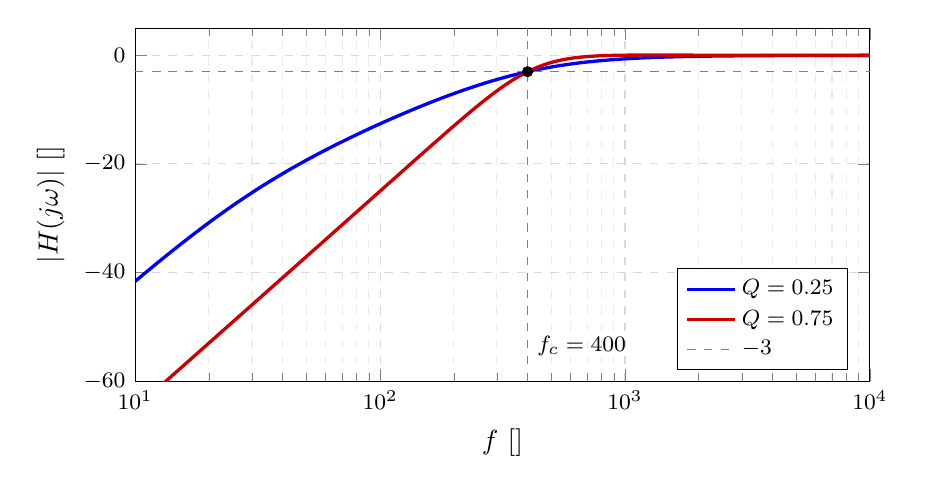
\begin{tikzpicture}
  \begin{semilogxaxis}[
    width=0.9\textwidth, height=0.5\textwidth,
    xlabel={$f$ [\unit{\hertz}]}, ylabel={$|H(j\omega)|$ [\unit{\decibel}]},
    xmin=10, xmax=10000, ymin=-60, ymax=5,
    grid=both, grid style={gray!30, dashed},
    minor grid style={gray!15, dashed},
    legend pos=south east, legend cell align=left, legend style={font=\footnotesize},
    tick label style={font=\footnotesize},
    samples=150, domain=10:10000, no marks,
  ]
    \addplot[blue, very thick]
      {20*log10((2*pi*x)^2 / sqrt((670.04^2 - (2*pi*x)^2)^2 + (670.04*2*pi*x/0.25)^2))};
    \addlegendentry{$Q = \num{0.25}$}
    \addplot[red!80!black, very thick]
      {20*log10((2*pi*x)^2 / sqrt((2656.40^2 - (2*pi*x)^2)^2 + (2656.40*2*pi*x/0.75)^2))};
    \addlegendentry{$Q = \num{0.75}$}
    \addplot[gray, dashed] {-3.01};
    \addlegendentry{$\qty{-3}{\decibel}$}
    \draw[dashed, gray] (axis cs:400,-60) -- (axis cs:400,5)
      node[pos=0.1, right, font=\footnotesize, black] {$f_c = \qty{400}{\hertz}$};
    \addplot[only marks, mark=*, mark size=1.8pt, black, forget plot] coordinates {(400,-3.01)};
  \end{semilogxaxis}
\end{tikzpicture}
